\subsection{Classification and Regression Trees}
\label{sec:CART}
The next 3 approaches all use a specific type of machine learning strategy to construct their predictors. This method is call Classification and Regression Tree's (\CART).
To create a \CART one first needs some data points. In the context of configurable software systems each point consists at least out of a configuration and an associated performance score. These data point are then fed into the algorithm seen in
 \cref{alg:CART}.
\begin{figure}
	\lstset{
		mathescape,
		breaklines=true,
	}
	\begin{lstlisting}
1. Start at the root node, add all data points to it.
2. For each option, find the set of options that minizes the sum of the node impurities in the two child nodes.
3. If a stopping criterion is reached, exit. Otherwise, apply step 2 to each child node inturn.
	\end{lstlisting}
	\captionof{lstlisting}{Pseudocode for generating a \CART. Adopted from \citet{ClassificationAndRegressionTrees}.}
	\label{alg:CART}
\end{figure}
\TODOX{beenden}

\begin{figure}
	\centering
	\includegraphics[page=4,clip,trim=3.5cm 18cm 3.5cm 1.5cm, width=\linewidth]
	{Paper/VariabilityAwarePerformancePredictionAStatisticalLearningApproach.pdf}
	\caption{Example performance model of X264 generated by CART based on the random sampling, using minimization of the sum of squared error loss \cite{VariabilityAwarePerformancePredictionJianmeiSigmundApel}.}	
	\label{fig:VAPPExampleTree}	
\end{figure}

